\documentclass[aspectratio=169,12pt]{beamer}
\usepackage{iftex}
\ifXeTeX
\usepackage{fontspec}
\defaultfontfeatures{Ligatures=TeX}
\setmainfont{Times New Roman}
\setsansfont{DejaVu Sans}
\setmonofont{DejaVu Sans Mono}
\else
\usepackage[T2A]{fontenc}
\usepackage[utf8]{inputenc}
\fi
\usepackage[russian]{babel}
\usepackage{amsmath}
\usepackage{graphicx}
\usepackage{array}
\usepackage{booktabs}
\graphicspath{{../prediploma_practice_report/images/}}

\usetheme{Madrid}
\usecolortheme{seahorse}
\usefonttheme{professionalfonts}
\setbeamertemplate{navigation symbols}{}
\setbeamertemplate{footline}[frame number]
\setbeamertemplate{headline}{}

\title{Разработка интерактивной программы\\визуализации движения частиц\\в полях скоростей}
\subtitle{Презентация по преддипломной практике}
\author{Гальчанский Данила Андреевич\\\small Руководитель: Ложников Михаил Андреевич}
\institute{МГУ имени М. В. Ломоносова\\Филиал в городе Душанбе}
\date{Душанбе, 2026}

\begin{document}

\begin{frame}
    \titlepage
\end{frame}

\begin{frame}{Актуальность, цель и задачи}
\begin{block}{Актуальность}
В задачах механики многофазных сред важно не только вычислить движение частиц,
но и быстро интерпретировать траектории в заданном поле скорости.
\end{block}

\begin{block}{Цель практики}
Разработать интерактивную программу, которая объединяет математическую модель
движения частицы и удобную визуализацию численного эксперимента.
\end{block}

\begin{itemize}
    \item проанализировать существующее расчётное ядро проекта;
    \item реализовать интерфейс выбора поля и запуска эксперимента;
    \item построить визуализацию линий тока, стрелок и траекторий;
    \item обеспечить устойчивую интерактивную работу программы.
\end{itemize}
\end{frame}

\begin{frame}{Математическая модель}
Рассматривается движение сферической частицы в двумерном поле скорости
$u(x,y) = (u_x, u_y)$. Основная учитываемая сила --- аэродинамическое сопротивление:

\begin{equation*}
    m\ddot q = F, \qquad
    F = \frac{\pi r^2}{2} C_d \rho |u-v|(u-v).
\end{equation*}

\begin{columns}[T]
\column{0.55\textwidth}
\begin{itemize}
    \item $q(t)$ --- положение частицы,
    \item $v(t)$ --- скорость частицы,
    \item $r$ --- радиус,
    \item $\rho$ --- плотность несущей среды,
    \item $C_d$ --- коэффициент сопротивления.
\end{itemize}

\column{0.45\textwidth}
Число Рейнольдса:
\begin{equation*}
    \mathrm{Re} = \frac{2\rho |u-v| r}{\mu}.
\end{equation*}

Коэффициент сопротивления:
\begin{equation*}
    C_d = \left(0.325 + \sqrt{0.124 + \frac{24}{\mathrm{Re}}}\right)^2.
\end{equation*}
\end{columns}
\end{frame}

\begin{frame}{Численная схема и визуализация}
\begin{itemize}
    \item Система движения частицы приводится к задаче первого порядка.
    \item Интегрирование выполняется методом Рунге--Кутты четвёртого порядка.
    \item Поле скорости задаётся встроенными аналитическими примерами или пользовательскими формулами.
    \item На сцене одновременно отображаются линии тока, стрелки поля, частицы и следы.
\end{itemize}

\begin{block}{Что даёт такой подход}
Пользователь видит не только геометрию течения, но и реальную инерционную реакцию
частицы на локальную структуру поля.
\end{block}
\end{frame}

\begin{frame}{Архитектура программы}
\small
\begin{columns}[T]
\column{0.58\textwidth}
\begin{itemize}
    \item \textbf{VectorField} --- вычисление скорости в произвольной точке области.
    \item \textbf{Particle} --- хранение состояния частицы и шаг интегрирования.
    \item \textbf{RenderWidget} --- отрисовка сцены, анимация, обработка мыши.
    \item \textbf{MainWindow} --- панель параметров и сценарий взаимодействия.
\end{itemize}

\begin{block}{Технологии}
Python, PySide6, QPainter, QTimer.
\end{block}

\column{0.42\textwidth}
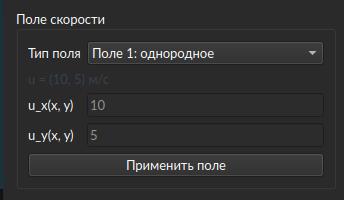
\includegraphics[width=0.94\linewidth]{field-params.png}
\vspace{0.5em}

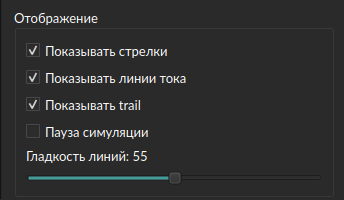
\includegraphics[width=0.94\linewidth]{view-params.png}
\end{columns}
\end{frame}

\begin{frame}{Интерфейс и пользовательский сценарий}
\scriptsize
\begin{columns}[T]
\column{0.54\textwidth}
Пользовательский сценарий:
\begin{itemize}
    \item выбрать встроенное поле или задать своё;
    \item настроить параметры частицы и отображения;
    \item добавить частицы щелчком или в режиме непрерывного источника;
    \item наблюдать траектории и сравнивать их с линиями тока.
\end{itemize}

\begin{itemize}
    \item слева --- управление,
    \item справа --- область численного эксперимента,
    \item интерфейс рассчитан на быстрый повтор сценариев.
\end{itemize}

\column{0.46\textwidth}
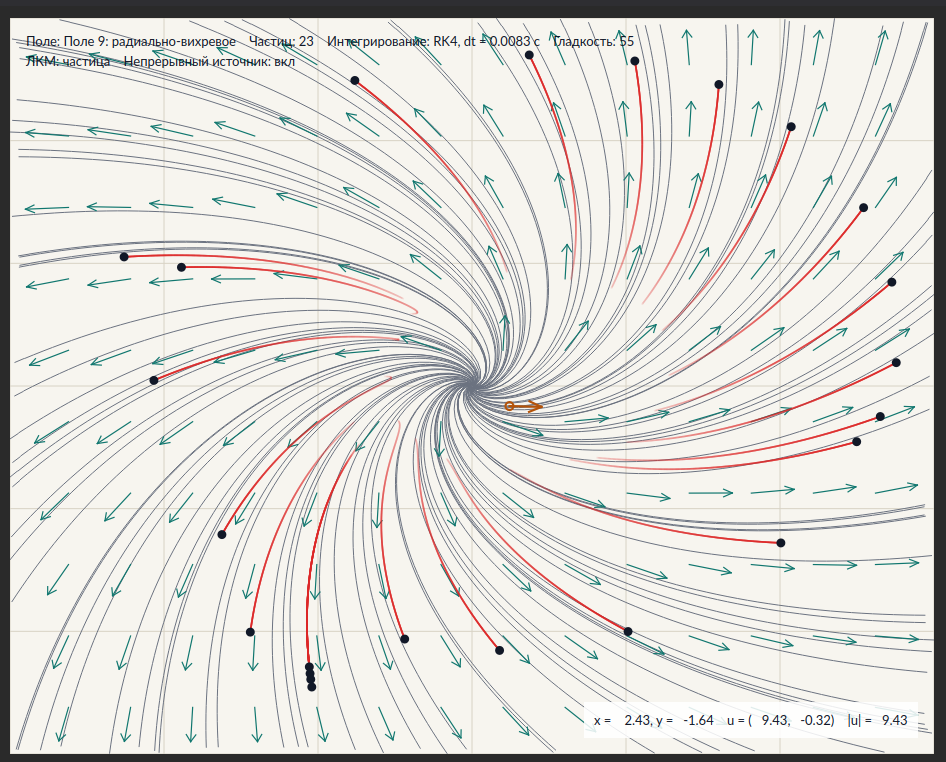
\includegraphics[width=0.9\linewidth]{field9-with-particles-hold-on.png}
\end{columns}
\end{frame}

\begin{frame}{Реализованные интерактивные функции}
\scriptsize
\begin{columns}[T]
\column{0.5\textwidth}
\begin{itemize}
    \item параметры частицы: радиус, плотность, начальная скорость;
    \item непрерывный источник при удержании левой кнопки мыши;
    \item fade-следы для наглядности траектории;
    \item локальная диагностика под курсором;
    \item сопоставление режимов движения при одном поле.
\end{itemize}

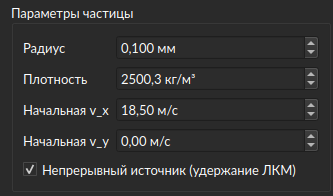
\includegraphics[width=0.72\linewidth]{particle-params.png}

\column{0.5\textwidth}
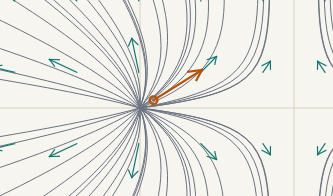
\includegraphics[width=0.62\linewidth]{velocity-vecor-under-cursor.png}

\vspace{0.5em}
\begin{block}{Практический эффект}
Программа стала инструментом для коротких интерактивных экспериментов.
\end{block}
\end{columns}
\end{frame}

\begin{frame}{Примеры численных экспериментов}
\scriptsize
\begin{columns}[T]
\column{0.5\textwidth}
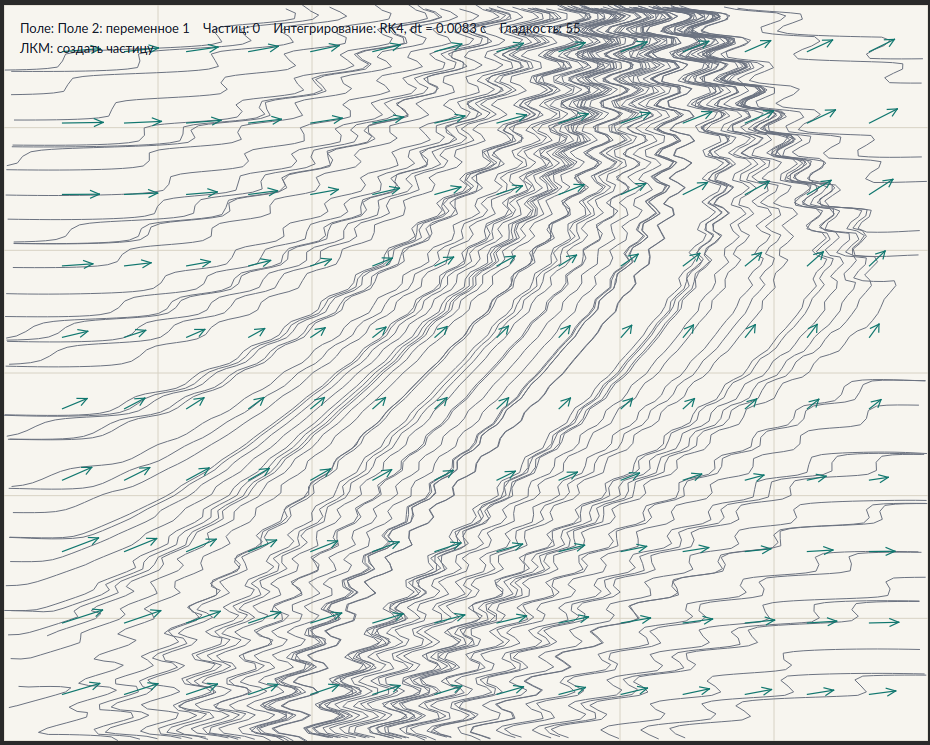
\includegraphics[height=0.37\textheight]{field2-viewer.png}

\vspace{0.3em}
\centering\small Поле скорости без частиц

\column{0.5\textwidth}
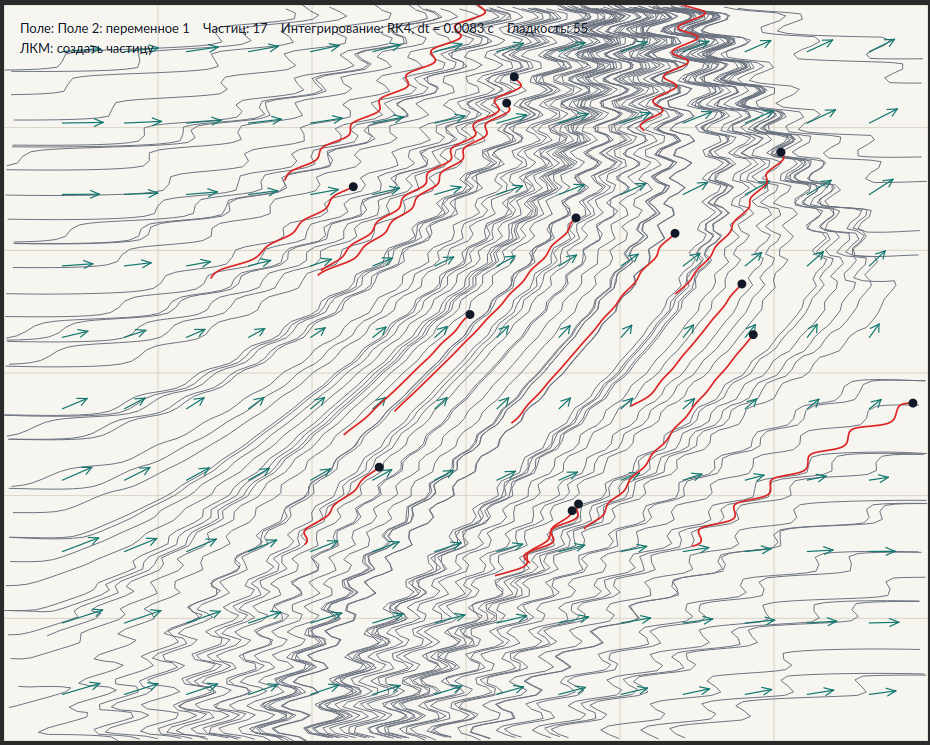
\includegraphics[height=0.37\textheight]{field2-with-particles-viewer.png}

\vspace{0.3em}
\centering\small То же поле с инерционными частицами
\end{columns}

\vspace{0.4em}
\begin{itemize}
    \item траектории не совпадают с линиями тока буквально;
    \item инерция частицы сглаживает локальные повороты потока.
\end{itemize}
\end{frame}

\begin{frame}{Инженерные результаты и устойчивость}
\small
\begin{itemize}
    \item добавлены проверки на нечисловые и экстремальные значения координат и скоростей;
    \item улучшено построение линий тока: больше стартовых точек и управление гладкостью;
    \item сохранён баланс между качеством визуализации и отзывчивостью интерфейса;
    \item поддержан пользовательский ввод аналитических формул поля.
\end{itemize}

\begin{block}{Итог}
Получена рабочая модульная система, пригодная для демонстрации, качественного
анализа и дальнейшего развития в рамках дипломного проекта.
\end{block}
\end{frame}

\begin{frame}{Основные результаты практики}
\begin{enumerate}
    \item Реализована интерактивная программа визуализации движения частиц в 2D-полях скорости.
    \item Перенесены в интерфейс математическая модель, тестовые поля и численные методы из дипломного проекта.
    \item Добавлены параметры частицы, непрерывный источник, fade-следы и диагностика под курсором.
    \item Подготовлена база для дальнейшего развития: новые модели, экспорт результатов, связь с расчётным ядром.
\end{enumerate}

\vfill
\begin{center}
\Large Спасибо за внимание
\end{center}
\end{frame}

\end{document}